\chapter{Projekt i jego implementacja}

Założeniami projektu opisanego w ninejszej pracy było stworzenie prototypu
oprogramowania umożliwiającego wykrywanie ataków DDoS w sieciach SDN oraz, co
ważniejsze, dającego się łatwo skalować w celu zwiększenia jego wydajności.
Wykorzystanie właściwej archtiektury rozwiązania oraz dobór odpowiednich
technologii do jego implementacji umożliwiły osiągnięcie zamierzonych celów.

\section{Architektura rozwiązania ochrony przed atakiem DDoS}

Projektując tytułowe rozwiązanie należało wziąć pod uwagę następujące czynniki:
\begin{itemize}
  \item umiejscowienie komponentu z oprogramowaniem w architekurze sieci SDN
  \item uzyskanie odpowiednich danych z sieci, pozwalających na wykrycie ataku
  \item wydajność działania oprogramowania
\end{itemize}

Oprogramowanie zostało zaprojektowane do działania na południowym interfejsie
architektury sieci SDN. Takie umiejscowienie dostarcza wielu możliwości.
Pierwszą z nich jest to, że oprogramowanie może być częścią przełącznika,
kontrolera lub działać na osobnym węźle. Dodatkowo oprogramowanie ma dostęp do
danych wymienianych pomiędzy przełącznikiem, a kontrolerem. Możliwość analizy
tychże danych była podstawą do implementacji algorytmu do wykrywania ataków DDoS
w sieci. Szczegóły dotycznące algorytmu zostały opisane w późniejszym rozdziale
ninejszej pracy. 

Wspomniane rozwiązanie zaimplementowano z myślą o działaniu na osobnym węźle,
ponieważ dzięki takiemu podejściu, w przypadku równoległego działania
oprogramowania, liczba jego instancji jest niezależna od liczby przełączników
lub kontrolerów. Dzięki temu, możliwe jest bardziej elastyczne skalowanie
horyzontalne oprogramowania w celu zwiększenia jego wydajności. Ponadto zarówno
przełączniki jak i kontroler nie są świadome obecności dodatkowego komponentu
pomiędzy nimi, co pozwala uniknąć dodatkowego narzutu związanego z konfiguracją
sieci SDN. 

Podstawowa topologia sieci SDN wraz z umiejscowionym komponentem reprezentującym
zaimplementowane oprogramowanie (\textit{sample component}) została
przedstawiona na Rys. \ref{fig:sdn_epc_flow}. 

\begin{figure}[h]
\centering
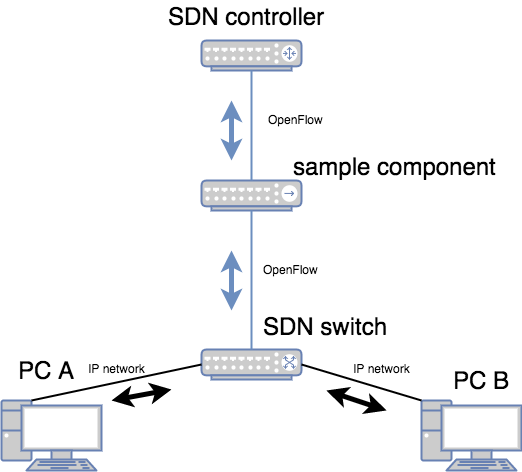
\includegraphics[width=\textwidth]{sdn_epc_flow}
\caption{Schemat podstawowej topologii sieciowej z umiejscowionym komponentem
  implementującym rozwiązanie projektowe}
\label{fig:sdn_epc_flow}
\end{figure}

Jak zostało przedstawione na Rys. \ref{fig:sdn_epc_flow} węzły końcowe
(\textit{PC N}) komunikują się ze sobą z wykorzystaniem przełącznika sieci SDN
(\textit{SDN switch}), a cały ruch pomiędzy przełącznikiem, a kontrolerem
(\textit{SDN controller}) przemieszcza się przez wspomniany komponent
implementujący rozwiązanie projektowe (\textit{sample component}).

Topologia zaprezentowana na Rys \ref{fig:sdn_epc_flow}, jak wspomniano, jest
tolopogią najbardziej podstawową, odpowiednią do wykorzystania prezentowanego
rozwiązania. Możliwe jest również, zastosowanie tego rozwiązania w bardziej
rozbudowanej sieci, składającej się z większej liczby węzłów końcowych, 
przełączników oraz kontrolerów. W takim przypadku, można zastosować kilka
instancji równlegle działającego oprogramowania (komponentu), w celu
zwiększenia wydajności systemu, rozumianego jako kilka współpracujących ze sobą
instancji. System taki, można zastosować do większych, pracujących pod większym
obciążeniem sieci. 

\section{Wybór odpowiednich technologii do implementacji systemu}

Podstawowym kryterium wyboru odpowiednich technologii do realizacji projektu
była wydajność. Wydajność jest rozumiana jako ilość pracy wykonana przez system
komputerowy w danym czasie i przy wykorzystaniu danej ilości zasobów
obliczeniowych \cite{distrforfunandprof}. Na potrzeby projektu, odpowiedni
poziom wydajności został zapewniony dzięki doborze techologi, które wspierają
koncepcję programowania współbieżnego, czyli możliwość wykonywania się
oprogramowania z wykorzytaniem wielu wątków fizycznych procesora maszyny, na
której zostało ono uruchomione. Ponadto, przy wyborze technologi, kierowano się
również natywnym wsparciem dla możliwosći dystrybucji oprogramowania na wiele
maszyn fizycznych, czyli, innymi słowy, wsparciem dla budowania systemów
rozproszonych. Możliwość rozbudowy systemu z wykorzystaniem wielu maszyn jest
kluczowa, ponieważ nawet dysponując technolgią ze wsparciem dla programowania
współbieżnego, istnieje granica dla rozbudowy zasobów sprzętowych, dlatego w
pewnym momencie koniecznym jest budowa systemu rozproszonego
\cite{distrforfunandprof}. 

Wykorzystanie technolgii, która umożliwa programowanie współbieżne oraz wspiera
budowę systemów rozporosznych, umożliwiło taką implementację projeku, która
pozwala na łatwe oraz efektywne jego skalowanie, celem zwiększenia wydajności.

Technologiami, które spełniają wszystkie wyżej wymienione wytyczne są funkcyjne
języki programowania Erlang oraz Elixir. Oba języki działają na Maszynie
Wirtualnej Erlanga (BEAM). W rzeczywistości Elixir jest nowoczesną wersją
Erlanga, dopasowaną do dzisiejszych standardów. Oferuje on szereg nowoczesnych,
ułatwiających pracę programistyczną narzędzi, których Erlang nie posiada. W
rzeczywistości Elixir jest Erlangową aplikacją działającą na Maszynie Wirtualnej
Erlanga \cite{thebeambook}.

Maszyna Wirtualna Erlanga wprowadza model aktorów
\footnote{https://en.wikipedia.org/wiki/Actor\_model}, dzięki czemu posiada
natywne wsparcie dla programowania równoległego. Ponadto, BEAM zapewnia
również wsparcie dla budowy systemów rozproszonych \cite{lyserlang}. Dzięki
temu, języki Erlang oraz Elixir są odpowiednie do budowy wydajnych,
niezawodnych, systemów rozproszonych. Z tych właśnie powodów, wspomniane
technologie zostały wykorzystane do budowy projektu przedstawionego w niniejszej
pracy.